% Draft Version 1 - Date 16/06/2020
% Draft Version 2 - Date 06/08/2020
% Draft Version 3 - Date 27/08/2020
% Draft Version 4 - Date 23/08/2020
\appendix
%\chapter{Appendix CH}
%\section{Kinematics}
%A body $  $
\chapter{Kinematics}\label{app-kine}
%The internal state vector $ \textbf{Z} $ is a vector that can be used to gather all the internal variable information of the constitutive behavior along with the deformation gradient $ \textbf{F} $, to get the observable quantity of the first Piola Kirchhoff stress tensor $ \textbf{P} $ by a general form
%\begin{equation}\label{app-kine-1}
%\textbf{P}(t)=\mathfrak{F}(\textbf{F}(t),Z(t))
%\end{equation}
%at any given time $ t $. 
Kinematics describes the transformation of a given material body from the reference state to the deformed state while not considering the reasons for the said deformation. The material is assumed to change its positions from $ \textbf{x} $ to $ \textbf{x}' $. The deformation tensor $ \textbf{F} $ is used to describe the deformation of an infinitesimal material volume in each point. The gradient operator relates the two states as
\begin{equation}\label{app-kine-1-1}
d\textbf{x}'=\textbf{F}\cdot d\textbf{x}
\end{equation}
in the form of 
\begin{equation}\label{app-kine-1-2}
\textbf{F}=\bm\nabla_0\textbf{x}'=\bm\nabla_0\textbf{x}+\bm\nabla_0\textbf{u}=\textbf{I}+\bm\nabla_0\textbf{u},
\end{equation}
where $ \textbf{u} $ is the displacement field. The determinant of the deformation tensor is always a positive number, since it is the quotient of two volumes, which mean that $ \textbf{F}^{-1} $ exists with $ J $ the Jacobian as $ J=\det F>0 $. Several rotation-independent deformation tensors are used in mechanics knowing that pure rotations do not induce strains in a deformable body. For example, the right Cauchy-Green stretch tensor $ \textbf{C} $ can be defined as
\begin{equation}\label{app-kine-6}
\textbf{C}=\textbf{F}^T\cdot\textbf{F}.
\end{equation}
The Green Lagrange strain tensor $ \textbf{E} $ can be defined as 
\begin{equation}\label{app-kine-8}
\textbf{E}=\frac{1}{2}(\textbf{C}-\textbf{I})=\frac{1}{2}(\textbf{U}^2-\textbf{I}).
\end{equation}
where $ \textbf{I} $ is an identity tensor. The tensor $ \textbf{C} $ is symmetric and positive definite, and has real valued eigenvectors that are orthogonal and positive eigenvalues allowing a spectral decomposition of $ \textbf{C} $.
The right stretch tensor $ \textbf{U} $, can be defined as
\begin{equation}\label{app-kine-7}
\textbf{U}=\sqrt{\textbf{C}}.
\end{equation}
It is obvious that $ \textbf{U} $ is also symmetric, positive definite and regular. The rotation tensor $ \textbf{R} $ is related by 
\begin{equation}\label{app-kine-7-1}
\textbf{R}=\textbf{F}\cdot\textbf{U}^{-1}.
\end{equation}
%Thus an assumption of frame indifference, $ \textbf{R}=\textbf{I} $ means $ \textbf{F}=\textbf{U} $. 
The left Cauchy-Green or the Finger deformation tensor $ \textbf{B} $ is defined as
\begin{equation}\label{app-kine-7-2}
\textbf{B}=\textbf{F}\cdot\textbf{F}^T.
\end{equation}

In standard analogy, by the conservation of angular momentum, one can write
\begin{equation}\label{app-kine-2}
\textbf{P}\cdot\textbf{F}^T=\textbf{F}\cdot\textbf{P}^T.
\end{equation}
From $ \textbf{F} $ and $ \textbf{P} $, one can obtain the Kirchhoff stress $ \boldsymbol\kappa $ as
\begin{equation}\label{app-kine-3}
\boldsymbol\kappa=\textbf{P}\cdot\textbf{F}^T.
\end{equation}
The Cauchy stress tensor or true stress tensor $ \bm\Sigma $ can be defined as 
\begin{equation}\label{app-kine-4}
\bm\Sigma=J^{-1}\boldsymbol\kappa.
\end{equation}
Finally, the $ 2^\text{nd} $-Piola Kirchhoff stress tensor $ \textbf{S} $, or PK2 can be then defined as
\begin{equation}\label{app-kine-5}
\textbf{S}=\textbf{F}^{-1}\cdot\textbf{P}.
\end{equation}

The tensors $ \textbf{S} $, $ \textbf{C} $, $ \textbf{U} $, and $ \textbf{E} $ are invariant and symmetric. 
%With the knowledge of the above relations, one can rewrite Eq. (\ref{app-kine-1} in the form that is appropriate for a given problem statement.


\chapter{J2-hyperelastic-based elasto-plastic material model}\label{app-j2}
\chaptermark{J2-hyperelastic}
In this part, the first Piola-Kirchhoff stress $ \textbf{P} $ and it work conjugate strain measure, the deformation gradient $ \textbf{F} $ are considered. Assuming a multiplicative decomposition of the deformation gradient gives
\begin{equation}\label{eq-j2-1}
\textbf{F}={\textbf{F} }^e {\textbf{F} }^p
\end{equation}
with $ \textbf{F}^e $ the elastic part and $ \textbf{F}^p $ the plastic part of the deformation gradient The elastic potential, on which the hyper-elasticity of the material model is based, is defined as
\begin{equation}\label{eq-j2-2}
\Psi({\textbf{C}}^e)=\frac{K}{2}\ln^2J+\frac{G}{4}[\ln{\textbf{C}}^e]^{\text{dev}}:[\ln{\textbf{C}}^e]^{\text{dev}},
\end{equation}
with the bulk modulus of the material $ K $, the shear modulus of the material $ G $, and the elastic right Cauchy strain tensor $ {\textbf{C}}^e={\textbf{F}^e}^T{\textbf{F}^e} $, and 
\begin{equation}\label{eq-j2-1-1}
K = \frac{E}{3(1-2\nu)},
\end{equation}
\begin{equation}\label{eq-j2-1-2}
G=\frac{E}{2(1+\nu)}.
\end{equation}
In Eq. (\ref{eq-j2-2}), $ \left[\ln{\textbf{C}}^e\right]^{dev} $ denotes the deviatoric part of $ \left[\ln{\textbf{C}}^e\right] $. The first Piola-Kirchhoff stress tensor can be expressed as 
\begin{eqnarray}
\textbf{P} & = & 2\textbf{F}\frac{\partial\Psi}{\partial\textbf{C}}=2\textbf{F}\left[{{\textbf{F}}^p}^{-1}\frac{\partial\Psi(\textbf{C}^e)}{\partial\textbf{C}^e}{{\textbf{F}}^p}^{-T}\right]\nonumber\\
& = & K\textbf{F}^{-T}\ln J+\textbf{F}^e\left[2G{\textbf{C}^e}^{-1}\cdot\left(\ln\sqrt{\textbf{C}^e}^\text{dev}\right)\right]{\textbf{F}^p}^{-T}.
\end{eqnarray}
The Kirchhoff stress, $ \boldsymbol\kappa=\textbf{P}\textbf{F}^T $, which is used to express the $ J_2 $-flow theory is given by
\begin{equation}\label{eq-j2-3}
\boldsymbol\kappa=p'\textbf{I}+\textbf{F}^e\left[2G{\textbf{C}}^{e-1}\cdot\left(\ln\sqrt{{\textbf{C}}^e}^\text{dev}\right)\right]\textbf{F}^{eT},
\end{equation}
with the pressure term $ p'= K\ln J$ and the second term on the right hand side representing the deviatoric part of the Kirchhoff stress $ \boldsymbol\kappa^\text{dev} $. Practically, plasticity is solved on the co-rotational space where the Kirchhoff stress $ \bm\kappa^\text{cor} $ reads
\begin{equation}\label{eq-j2-2-1}
\bm\kappa^\text{cor}=p'\textbf{I}+2G\ln\sqrt{\textbf{C}^e}^\text{dev}.
\end{equation}
%with the von Mises stress $ \tau_e=\textbf{F}^e\textbf{C}^{e-1}\bm\kappa\textbf{F}^{eT} $. 
%\subsection*{Associated Flow Rule} 
Denoting $ {\bm\kappa^\text{dev}}^\text{cor}=2G\ln\sqrt{\textbf{C}^e}^\text{dev} $, the von Mises stress reads $ \kappa^\text{eq}=\sqrt{\frac{3}{2}{\bm\kappa^\text{dev}}^\text{cor}:{\bm\kappa^\text{dev}}^\text{cor}} $. 
From $ J_2 $-elasto-plasticity theory\cite{borjaPlasticityModelingComputation2013}, the von Mises stress criterion is given by
\begin{equation}\label{eq-j2-4}
f=\kappa^{\text{eq}}-R(p)-\sigma^0_y\le0
\end{equation}
with the yield surface $ f $, the equivalent von Mises stress $ \kappa^\text{eq} $, the initial yield stress $ \sigma^0_y $ and the isotropic hardening stress $ R(p)\ge0 $. The internal variable $ p $ is the equivalent plastic strain that characterizes the irreversible behavior. The normal plastic flow that follows from Eq. (\ref{eq-j2-4}) gives the incremental plastic deformation gradient between the two time-step configurations $ n $ and $ n+1 $,
\begin{equation}\label{eq-j2-4-5}
{\textbf{F}^{\text{p}}}_{n+1}=\text{exp}(\Delta p\mathbf{N}^{\text{p}})\cdot{\textbf{F}^{\text{p}}}_n,
\end{equation}
\begin{equation}\label{eq-j2-4-6}
%of \mathbf{N}^{\text{p}}=\frac{\partial f}{\partial \bm{\sigma}}=\frac{3}{2}\frac{\bm{\boldsymbol\tau}^\text{dev}}{\tau^\text{eq}}.
\mathbf{N}^{\text{p}}=\frac{\partial f}{\partial \bm{\kappa}^\text{cor}}=\frac{3}{2}\frac{{\bm{\kappa}^\text{dev}}^\text{cor}}{\kappa^\text{eq}}.
\end{equation}
One can define the plastic strain rate tensor $ \bm\varepsilon^p $ using the flow rule by
\begin{equation}\label{eq-j2-4-2}
\bm\varepsilon^p=\overset{.}{ \textbf{F}}^p\cdot{\textbf{F}^p}^{-1}=\dot\lambda\mathbf{N}^{\text{p}}
\end{equation}
which is the result of applying the Clausius-Duhem inequality and $ \lambda $ is the plastic multiplier. From the Karush-Kuhn-Tucker condition, it can be shown that the loading-unloading consistency condition is equivalent to 
\begin{equation}\label{eq-j2-4-3}
\dot\lambda\ge0,f\le0,\dot\lambda f=0.
\end{equation}
Finally, the evolution of the equivalent plastic strain rate can be based on the isotropic hardening stress as
\begin{equation}\label{eq-j2-4-4}
\kappa^\text{eq}=R(p)+\sigma_y^0,
\end{equation}
\begin{equation}\label{eq-j2-5}
\dot{p}=\sqrt{\frac{2}{3}\bm\varepsilon^p:\bm\varepsilon^p}=\dot\lambda.
\end{equation}
The related close form expressions and the resolution of the system of Eqs. (\ref{eq-j2-1}) - (\ref{eq-j2-5}) are further explained in \cite{cuitinoMaterialindependantMethodExtending1992} and \cite{nguyenComputationalHomogenizationCellular2014}.

%\subsection*{Non-associated Flow Rule} \cite{nguyenLargeStrainHyperelastic2016}
%\section{Finite element functions}

\chapter{State based representation}\label{app-state}
%\chaptermark{State}
From the definition of the elastic right Cauchy strain tensor $ \textbf{C}^e={\textbf{F}^e}^T\cdot\textbf{F}^e $, one can deduce
\begin{equation}\label{app-state-1}
\textbf{C}^e={\textbf{F}^p}^{-T}\cdot\textbf{C}\cdot{\textbf{F}^p}^{-1}.
\end{equation}
This gives
\begin{equation}\label{app-state-2}
\overset{.}{\textbf{C}}={\overset{.}{\textbf{F}}^p}^T\cdot\textbf{C}^e\cdot\textbf{F}^p+{\overset{}{\textbf{F}}^p}^T\cdot\textbf{C}^e\cdot\overset{.}{\textbf{F}^p}+{\overset{}{\textbf{F}}^p}^T\cdot\overset{.}{\textbf{C}^e}\cdot\overset{}{\textbf{F}^p}.
\end{equation}
Using a flow rule similar to the one described in Eq. (\ref{eq-j2-4-2}), one can rewrite Eq. (\ref{app-state-2}) for an appropriate J2-hyper-elastic based constitutive law as
\begin{equation}\label{app-state-3}
\overset{.}{\textbf{C}^e}={\textbf{F}^p}^{-T}\cdot\overset{.}{\textbf{C}}\cdot{\textbf{F}^p}^{-1}-\dot\lambda(\textbf{N}^p\cdot\textbf{C}^e+\textbf{C}^e\cdot\textbf{N}^p).
\end{equation}
In finite plasticity, the Mandel stress, $ \textbf{M}^e $, is the energetically conjugate stress of the logarithmic strain measure $ \ln\sqrt{\textbf{C}^e} $ which can be defined as 
\begin{eqnarray}\label{app-state-4}
\textbf{M}^e = \frac{1}{2}(\textbf{C}^e\cdot\textbf{S}+\textbf{S}\cdot\textbf{C}^e)= 2\textbf{C}^e\cdot\frac{\partial\Psi}{\partial\textbf{C}^e} = \mathbb{C}:\ln\sqrt{\textbf{C}^e}=\bm\kappa^\text{cor},
\end{eqnarray}
where we have assumed commutativity of $ \textbf{C}^e $ and $ \textbf{S} $, and $ \mathbb{C} $ is the Hook tensor, defined as
\begin{equation}\label{app-state-4-1}
\mathbb{C}=\left(K-\frac{2G}{3}\right)\textbf{I}\otimes\textbf{I}+G\textbf{I}.
\end{equation}
The consistency condition (\ref{eq-j2-4-3}) during plasticity can be written as a function of $ \textbf{C}^e $ and  $ \lambda $ considering that they respectively are the factors of $ \textbf{M}^e $ and $ f $ in the following manner
\begin{equation}\label{app-state-5}
\frac{\partial f}{\partial \textbf{C}^e}:\overset{.}{\textbf{C}^e}+\frac{\partial f}{\partial p}\dot{p}=0,
\end{equation}
where the explicit forms of $ f $ and $ R(p) $ yield
\begin{equation}\label{app-state-6}
\frac{\partial f}{\partial \textbf{C}^e}=\frac{\partial f}{\partial \textbf{M}^e}:\frac{\partial\textbf{M}^e}{\partial \textbf{C}^e}=\textbf{N}^p:\frac{\partial\textbf{M}^e}{\partial \textbf{C}^e}
\end{equation}
and 
\begin{equation}\label{app-state-7}
\frac{\partial f}{\partial p}=\frac{\partial f}{\partial R(p)}\frac{\partial R(p)}{\partial p}=-\frac{\partial R}{\partial p}.
\end{equation}
One can now write Eq. (\ref{app-state-5}) from Eqs. (\ref{app-state-3}) and (\ref{eq-j2-5}) as
\begin{equation}\label{app-state-8}
\frac{\partial f}{\partial \textbf{C}^e}:\left[{\textbf{F}^p}^{-T}\cdot\overset{.}{\textbf{C}}\cdot{\textbf{F}^p}^{-1}-\dot\lambda(\textbf{N}^p\cdot\textbf{C}^e+\textbf{C}^e\cdot\textbf{N}^p)\right]+\frac{\partial f}{\partial p}\dot\lambda=0,
\end{equation}
and Eq. (\ref{app-state-8}) can then be rewritten as 
\begin{equation}\label{app-state-9}
\dot\lambda=\textbf{A}:\overset{.}{\textbf{C}},
\end{equation}
where $ \textbf{A} $ represents a function of $ \textbf{C}^e $, $ \textbf{F}^p $ and $ p $ in the form of
\begin{equation}\label{app-state-10}
\textbf{A}=\frac{{\textbf{F}^p}^{-1}\cdot\left(\textbf{N}^p:\frac{\partial\textbf{M}^e}{\partial\textbf{C}^e}\right)\cdot{\textbf{F}^p}^{-T}}{\textbf{N}^p:\left(2\frac{\partial\textbf{M}^e}{\partial\textbf{C}^e}\cdot\textbf{C}^e\right):\textbf{N}^p+\frac{\partial R}{\partial p}}
\end{equation}
This gives a general choice for internal state variables as 
\begin{equation}\label{app-state-11}
\textbf{Z}=\left[
\begin{array}{c}
{\textbf{F}^p} \\ p
\end{array}
\right].
\end{equation}
The loading conditions help in defining the rate of change of state representation in the following manner,
\begin{equation}\label{app-state-12}
\overset{.}{\textbf{Z}} = 
\begin{cases}
	\begin{array}{c c}
		0 & \text{ if }f<0 \\
		\left[
			\begin{array}{c}
				\left[\left(\textbf{N}^p\cdot\textbf{F}^p\right)\otimes\textbf{A}\right]:\overset{.}{\textbf{C}} \\
				\textbf{A}:\overset{.}{\textbf{C}}
			\end{array}
		\right] & \text{ if }f=0
	\end{array}
\end{cases}.
\end{equation}

\chapter{Finite element formulation}\label{app-fem}
In the finite element (FE) method, the domain is initially discretized into elements with finite number of degrees of freedom, i.e. $ \Omega=\bigcup_e\Omega_0^e $. Similarly, the boundaries are also discretized, i.e. $ \partial_N\Omega\approx\bigcup\Gamma_0^e $. The FE approximation discretizes the displacement $ \textbf{u} $ over any given element $ \Omega_0^e $ as
\begin{equation}\label{app-fem-1}
\textbf{u(X)}=\sum_aN_a^e(\textbf{X})\textbf{u}_a=\textbf{N}^e\textbf{u}^e.
\end{equation}
$ N^e_a $ represents the nodal shape functions whereas $ \textbf{u}_a $ represents the unknown displacement associated to a node $ a $. The shape functions and unknowns can all be gathered into the elementary matrix $ \textbf{N}^e $ and vector $ \textbf{u}^e $ respectively.

The minimization problem from the balance of equilibrium or the unconstrained parts in Eqs (\ref{eq-res-1}) and (\ref{eq-res-2}) leads one to the minimization of the residual force vector $ \textbf{r}(\textbf{u}_\Omega) $ such that
\begin{equation}\label{app-fem-2}
\textbf{r}(\textbf{u}_\Omega)=\textbf{f}_\text{int}-\textbf{f}_\text{ext}=0.
\end{equation}
Here the internal forces $ \textbf{f}_\text{int} $ are given by
\begin{equation}\label{app-fem-3}
\textbf{f}_\text{int}(\textbf{u}_\Omega)=\underset{\Omega_0^e\subset\Omega}{\bigwedge}\int_{\Omega_0^e}(\textbf{B}^e)^T\textbf{P}\ dV
\end{equation}
and the external forces as
\begin{equation}\label{app-fem-4}
\textbf{f}_\text{ext}=
%\underset{\Omega_0^e\subset\Omega}{\bigwedge}\int_{\Omega_0^e}(\textbf{N}^e)^T\ dV+
\underset{\Gamma_0^e\subset\partial_N\Omega}{\bigwedge}\int_{\Gamma_0^e}(\textbf{N}^e)^T\textbf{T}^0\ dA.
\end{equation}
Here $ \bigwedge $ indicates the matrix assembly, $ \textbf{B}^e $ the elementary matrices of the gradient of the shape functions associated to the displacement field vector and $ \textbf{u}_\Omega=\bigwedge_{\Omega_0^e\subset\Omega}\textbf{u}^e $ is the vector that gathers all the elementary unknowns over $ \Omega $.

The system represented in Eq. (\ref{app-fem-2}) can be resolved by a standard Newton Raphson iterative procedure where the unknown vector $ \textbf{u}_\Omega $ is updated at each iteration by
\begin{equation}\label{app-fem-5}
\Delta\textbf{u}_\Omega=-\textbf{K}^{-1}\textbf{r}
\end{equation}
where $ \textbf{K} $ is the stiffness matrix defined as
\begin{equation}\label{app-fem-6}
\textbf{K}=\bigwedge_{\Omega_0^e\subset\Omega}\int_{\Omega_0^e}(\textbf{B}^e)^T\textbf{L}(\textbf{B}^e)\ dV
\end{equation}
with the material tangent operator $ \textbf{L} $ as
\begin{equation}\label{app-fem-7}
\textbf{L}=\frac{\partial\textbf{P}}{\partial\textbf{F}}
\end{equation}
The constitutive laws is used to deduce the relationships between the deformation tensor $ \textbf{F} $, the Piola-Kirchhoff stress tensor $ \textbf{P} $ and the tangent operator $ \textbf{L} $.

\chapter{Angle based representation}\label{app-angle}

\begin{figure}
	\centering
	\begin{subfigure}{0.45\textwidth}
		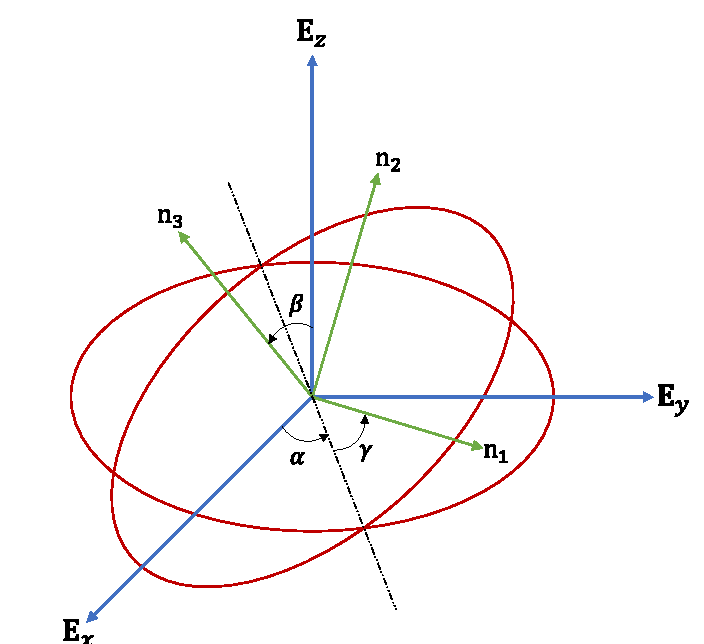
\includegraphics[width=\textwidth]{angle_rep_1}
		\caption{}
	\end{subfigure}
	\begin{subfigure}{0.45\textwidth}
	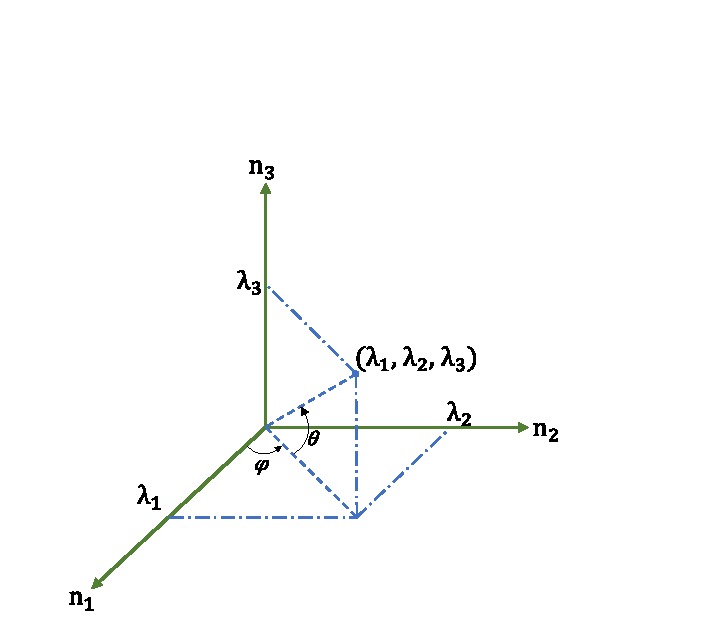
\includegraphics[width=\textwidth]{angle_rep_2}
	\caption{}
\end{subfigure}
\caption{(a) Transformation from current space to the eigenspace by the help of Euler angles; (b) Paramterization of eigenvalues in the principle space.}\label{app-angle-fig}
\end{figure}

Any arbitrary second order symmetric tensor $ \textbf{A} $ can undergo a spectral decomposition into its eigenvalues, $ \lambda_i $ and eigenvectors, $ \textbf{n}_i $ as
\begin{equation}\label{app-angle-1-1}
\textbf{A} = \textbf{Q}^T\boldsymbol\Lambda\textbf{Q},
\end{equation}
where $ \textbf{Q} $ is the orthogonal matrix whose columns are the eigenvectors and $ \boldsymbol\Lambda $ is a diagonal matrix with the eigenvalues as the entries. Thus,
\begin{equation}\label{app-angle-1}
\textbf{A}=\lambda_1\textbf{n}_1\otimes\textbf{n}_1+\lambda_2\textbf{n}_2\otimes\textbf{n}_2+\lambda_3\textbf{n}_3\otimes\textbf{n}_3.
\end{equation}
Considering that the eigenvectors $ \textbf{n}_1 $, $ \textbf{n}_2 $ and $ \textbf{n}_3 $ form an orthogonal basis, the transformation from current space $ (\textbf{E}_x,\textbf{E}_y,\textbf{E}_z) $ to eigen basis space $ (\textbf{n}_1,\textbf{n}_2,\textbf{n}_3) $ can be parametrized with the help of the three Euler angles $ \alpha $, $ \beta $ and $ \gamma $ (Figure \ref{app-angle-fig}(a)), as follows
\begin{equation}\label{app-angle-2}
\textbf{n}_1=\left[
\begin{array}{c}
\cos\gamma\cos\alpha-\cos\beta\sin\alpha\sin\gamma\\
\cos\gamma\sin\alpha+\cos\beta\cos\alpha\sin\gamma\\
\sin\beta\sin\gamma
\end{array}
\right],
\end{equation}
\begin{equation}\label{app-angle-3}
\textbf{n}_2=\left[
\begin{array}{c}
-\sin\gamma\cos\alpha-\cos\beta\sin\alpha\cos\gamma\\
-\sin\gamma\sin\alpha+\cos\beta\cos\alpha\cos\gamma\\
\sin\beta\cos\gamma
\end{array}
\right],
\end{equation}
and
\begin{equation}\label{app-angle-4}
\textbf{n}_3=\left[
\begin{array}{c}
\sin\beta\sin\alpha\\
-\sin\beta\cos\alpha\\
\cos\beta
\end{array}
\right],
\end{equation}
such that $ \alpha\in\left[0\ 2\pi\right] $, $ \beta\in\left[0\ \pi\right] $ and $ \gamma\in\left[0\ \frac{\pi}{2}\right] $. It is also possible to obtain the magnitude of $ \textbf{A} $ as
\begin{eqnarray}\label{app-angle-5}
||\textbf{A}|| & = & \sqrt{\textbf{A}:\textbf{A}}\\
 & = & \sqrt{\lambda_1^2+\lambda_2^2+\lambda_3^2}.
\end{eqnarray}
In the orthogonal eigen basis (Figure \ref{app-angle-fig}(b)), $ \lambda_1 $, $ \lambda_2 $ and $ \lambda_3 $ can be represented in the parametric form with the help of $ \theta $ and $ \varphi $ as 
\begin{equation}\label{app-angle-6}
\lambda_1=||\textbf{A}||\cos\theta\cos\varphi,
\end{equation}
\begin{equation}\label{app-angle-7}
\lambda_2=||\textbf{A}||\cos\theta\sin\varphi,
\end{equation}
and
\begin{equation}\label{app-angle-8}
\lambda_3=||\textbf{A}||\sin\theta,
\end{equation}
such that $ \theta\in\left[\frac{-\pi}{2}\ \frac{\pi}{2}\right] $ and $ \varphi\in\left[0\ 2\pi\right] $. With the help of the magnitude and the 5 angles, one can represent any given tensor $ \textbf{A} $ using the angle representation notation as
\begin{equation}\label{app-angle-9}
\hat{\textbf{A}}(\textbf{A})=\left[||\textbf{A}||\ \varphi\ \theta\ \alpha\ \beta\ \gamma\right].
\end{equation}
This formulation represents an efficient way to diagonalize a real symmetric matrix and store it in a digital form. The inverse operator $ \hat{\textbf{A}}^{-1} $ can be used to recover the original tensor $ \textbf{A} $ as
\begin{equation}\label{app-angle-11}
\textbf{A}=\hat{\textbf{A}}^{-1}\left(\left[||\textbf{A}||\ \varphi\ \theta\ \alpha\ \beta\ \gamma\right]\right).
\end{equation}

In 2 dimensional case, the parametrization reduces to
\begin{equation}\label{app-angle-10}
\hat{\textbf{A}}(\textbf{A})=\left[||\textbf{A}||\ \varphi\ \alpha\right],
\end{equation}
as 
\[ \theta=\beta=\gamma=0, \]
and the inverse operator is
\begin{equation}\label{app-angle-12}
\textbf{A}=\hat{\textbf{A}}^{-1}\left(\left[||\textbf{A}||\ \varphi\ \alpha\ \right]\right).
\end{equation}

\chapter{Activation functions}\label{app-act}
Activation functions in ANN are used to define the outputs of a given particular node for the given input. In general, these functions can be seen as an "ON" (1) and "OFF" (0) switch that is activated depending on the input. It is very important for an activation function to be computationally efficient so that thousans or even millions of them can be calculated at each neuron for every data sample that is given as an input. It could be a simple step function or a transformation that maps the input signals into the output signals that are necessary for the ANN to function. Here, some of the common activation functions that are used in standard neural networks, and their benefits and shortcomings are described in brief.

\paragraph*{Binary step function} represents a simple threshold-based activation function that activates based on a certain threshold sending exactly the same value as the signal to the next layer, like
\begin{equation}\label{app-act-1}
\phi_{BIN}(\nu)=
\begin{cases}
0\quad\text{ for }\nu<0\\
1\quad\text{ for }\nu\ge0\\
\end{cases}
\end{equation}
However this simple activation function cannot allow multi-value outputs.

\begin{figure}
	\centering
	\begin{subfigure}{0.45\textwidth}
		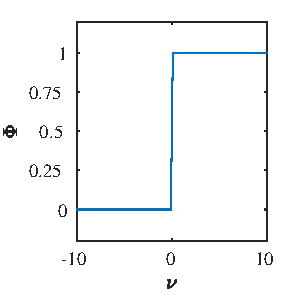
\includegraphics[]{act_binary}
		\caption{}
	\end{subfigure}
	\begin{subfigure}{0.45\textwidth}
		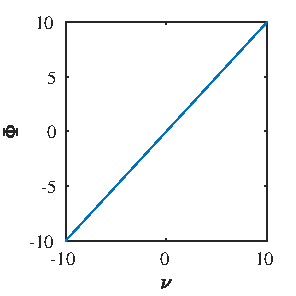
\includegraphics[]{act_linear}
		\caption{}
	\end{subfigure}
	\caption{(a) Binary activation function; (b) Linear activation function.}
\end{figure}

\paragraph*{Linear activation function} can simply take the form
\begin{equation}\label{app-act-2}
\phi_{LIN}(\nu)=\epsilon\nu
\end{equation}
where $ \epsilon $ is a constant. This results in a proportional output compared to the input, thus allowing multiple outputs, and not simply a 0 or 1. The derivation of $ \phi_{LIN} $ is
\begin{equation}\label{app-act-3}
\phi_{LIN}'(\nu)=\epsilon.
\end{equation}

Since $ \phi_{LIN}'(\nu) $ is a constant and has no relation to the input, linear functions can not be used for backpropagation using gradient descent as described in Eq. (\ref{eq-nn-sgd2}) and Section \ref{nn-ann-train}. This obstructs the model from going back in the network and understanding which are the possible weights that enables a better prediction. Another trivial problem of using a linear activation function is that the entire combinations of layers can be collapsed into one since a combination of linear functions is still linear in nature. Thus the neural network is simply a regression model with limited ability to handle complex inputs and parameters.

To ensure the ability of backpropagation with existing derivatives and the ability to use stacked layers to create deeper networks, one needs to look into non linear activation functions with sufficient complexity.

\paragraph*{Sigmoid or logistic activation function} gives an S-shaped curve that is followed by 
\begin{equation}\label{app-act-4}
\phi_{SIG}(\nu)=\frac{\text{e}^\nu}{\text{e}^\nu+1}.
\end{equation}
The derivative of $ \phi_{SIG}(\nu) $ is
\begin{equation}\label{app-act-4-1}
\phi_{SIG}'(\nu)=\phi_{SIG}(\nu)(1-\phi_{SIG}(\nu)).
\end{equation}
It ensures a smooth gradient while ensuring that the range of output stays between 0 and 1, thus ensuring normalized behavior of the neuron. This function ensures clear predictions at the edge of the curve, for $ \nu>2 $ or $ \nu<-2 $. However this also means that at such high values of input the resulting change in predictions is negligible introducing a vanished gradient.

\begin{figure}
	\centering
	\begin{subfigure}{0.45\textwidth}
		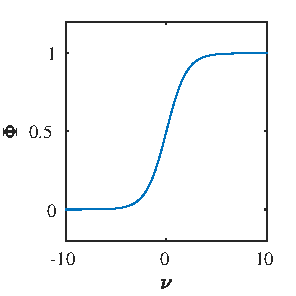
\includegraphics[]{act_sigmoid}
		\caption{}
	\end{subfigure}
	\begin{subfigure}{0.45\textwidth}
		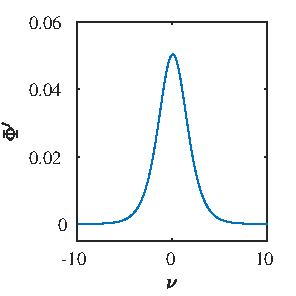
\includegraphics[]{act_sigmoid_diff}
		\caption{}
	\end{subfigure}
	\caption{(a) Sigmoid activation function; and (b) its derivative.}
\end{figure}

\paragraph*{Hyperbolic tangent activation function} or the TANH operator is defined by 
\begin{equation}\label{app-act-5}
\phi_{TANH}(\nu)=\tanh(\nu)=\frac{\left(\text{e}^\nu-\text{e}^{-\nu}\right)}{\text{e}^{\nu}+\text{e}^{-\nu}}.
\end{equation}
The derivative of $ \phi_{TANH} $ is
\begin{equation}\label{app-act-5-1}
\phi_{TANH}'(\nu)=1-\phi_{TAN}(\nu)^2.
\end{equation}
Compared to $ \phi_{SIG} $, $ \phi_{TANH} $ is zero centered allowing a strong ranges to be modeled easily. However both $ \phi_{SIG} $ and $ \phi_{TANH} $ are computationally expensive.

\begin{figure}
	\centering
	\begin{subfigure}{0.45\textwidth}
		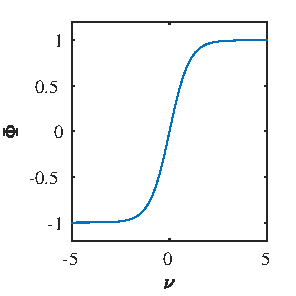
\includegraphics[]{act_tanh}
		\caption{}
	\end{subfigure}
	\begin{subfigure}{0.45\textwidth}
		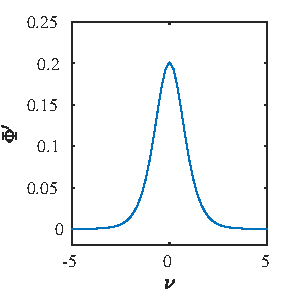
\includegraphics[]{act_tanh_diff}
		\caption{}
	\end{subfigure}
	\caption{(a) Hyperbolic tangent activation function; and (b) its derivative.}
\end{figure}

\paragraph*{Rectified linear unit based activation function} is defined as the positive part of the input argument,
\begin{equation}\label{app-act-6}
\phi_{RELU}(\nu)=
\begin{cases}
\nu,\quad \nu\ge0\\
0,\quad \nu<0
\end{cases}
\end{equation}
with its derivative being
\begin{equation}\label{app-act-6-1}
\phi_{RELU}'(\nu)=
\begin{cases}
1,\quad \nu\ge0\\
0,\quad \nu<0
\end{cases}.
\end{equation}
The simple looking function, that behaves like a ramp function, is computationally quite efficient and converges very quickly compared to the other activation functions. The ReLU is still a nonlinear function that can be used for backpropagation algorithms. However, when the inputs go close to, or below 0, the 0 gradient does not let the model learn further, a situation known as dying ReLU problem.

\begin{figure}
	\centering
	\begin{subfigure}{0.45\textwidth}
		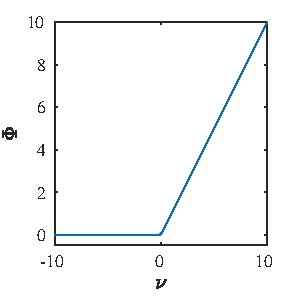
\includegraphics[]{act_relu}
		\caption{}
	\end{subfigure}
	\begin{subfigure}{0.45\textwidth}
		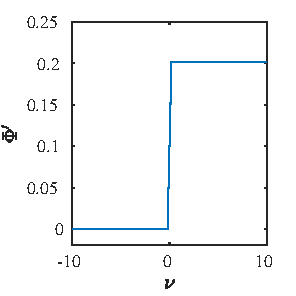
\includegraphics[]{act_relu_diff}
		\caption{}
	\end{subfigure}
	\caption{(a) Rectified linear unit activation function; and (b) its derivative.}
\end{figure}

\paragraph*{Leaky ReLU activation function} is a modified rectifier unit that behaves in the following manner
\begin{equation}\label{app-act-7}
\phi_{LR}(\nu)=
\begin{cases}
\nu,\quad \nu\ge0\\
\epsilon\nu,\quad \nu<0
\end{cases}
\end{equation}
where $ \epsilon $ is a small scalar value. The derivative of $ \phi_{LR} $ is
\begin{equation}\label{app-act-7-1}
\phi_{LR}'(\nu)=
\begin{cases}
1,\quad \nu\ge0\\
\epsilon,\quad \nu<0
\end{cases}
\end{equation}
thus solving the problem of dying ReLU.

\begin{figure}
	\centering
	\begin{subfigure}{0.45\textwidth}
		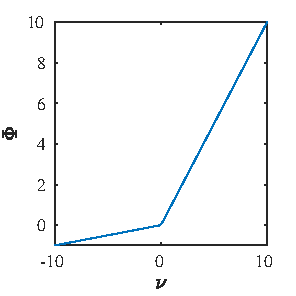
\includegraphics[]{act_lrelu}
		\caption{}
	\end{subfigure}
	\begin{subfigure}{0.45\textwidth}
		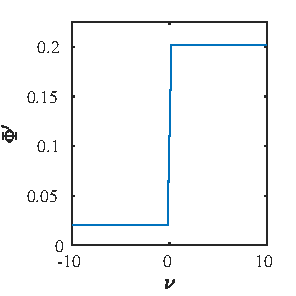
\includegraphics[]{act_lrelu_diff}
		\caption{}
	\end{subfigure}
	\caption{(a) Leaky ReLU activation function; and (b) its derivative.}
\end{figure}

\paragraph*{Softmax activation function} is a normalized exponential function that normalizes the input argument into a probablity distribution proportional to the exponential of the input numbers. It can be used in the output layer for classification problem, since it gives a 0 or 1 output for each category. It can be defined as 
\begin{equation}\label{app-act-8}
\phi_{SM_i}(\bm\nu)=\frac{\text{e}^{\nu_i}}{\sum_{j=1}^{J}\text{e}^{\nu_j}}\quad\text{for }i=1,...,J\text{ and }\bm\nu=(\nu_1,...,\nu_J)\in\mathbb{R}^J
\end{equation}
with its derivative being
\begin{equation}\label{app-act-8-1}
\frac{\partial\phi_{SM_i}(\bm\nu)}{\partial\nu_j}=\phi_{SM_i}(\bm\nu)(\delta_{ij}-\phi_{SM_j}(\bm\nu))
\end{equation}
where $ \delta_{ij} $ is the Kronecker delta,
\[ \delta_{ij}=\begin{cases}
1\quad\text{if }i=j\\
0\quad\text{if }i\ne j.
\end{cases} \]

The activation functions can be chosen depending on the type of neural networks that needs to be constructed along with the type of problem statement that needs to be trained for. In general the ReLU and its extension, leaky ReLU, are well suited for regression problems with a lot of continuous data whereas softmax function can be well suited for a classification type of problem.

\chapter{Description of Specific RNN networks}\label{app-lstm}
\paragraph*{Long Short Term Memory (LSTM)} To get around the problem of long term dependencies, when the RNNs become unable to connect past information due to a large gap between the two events, networks based on LSTM cells were introduced by Hochreiter \& Schmidhuber\cite{hochreiterLongShortTermMemory1997} and this has been briefly mentioned in Chapter \ref{chap-nn}. Each LSTM module is made of four neural network layers, interacting with each other in a very special way (Figure \ref{app-lstm-detail}).

\begin{figure}
	\centering
	\begin{subfigure}{0.98\textwidth}
		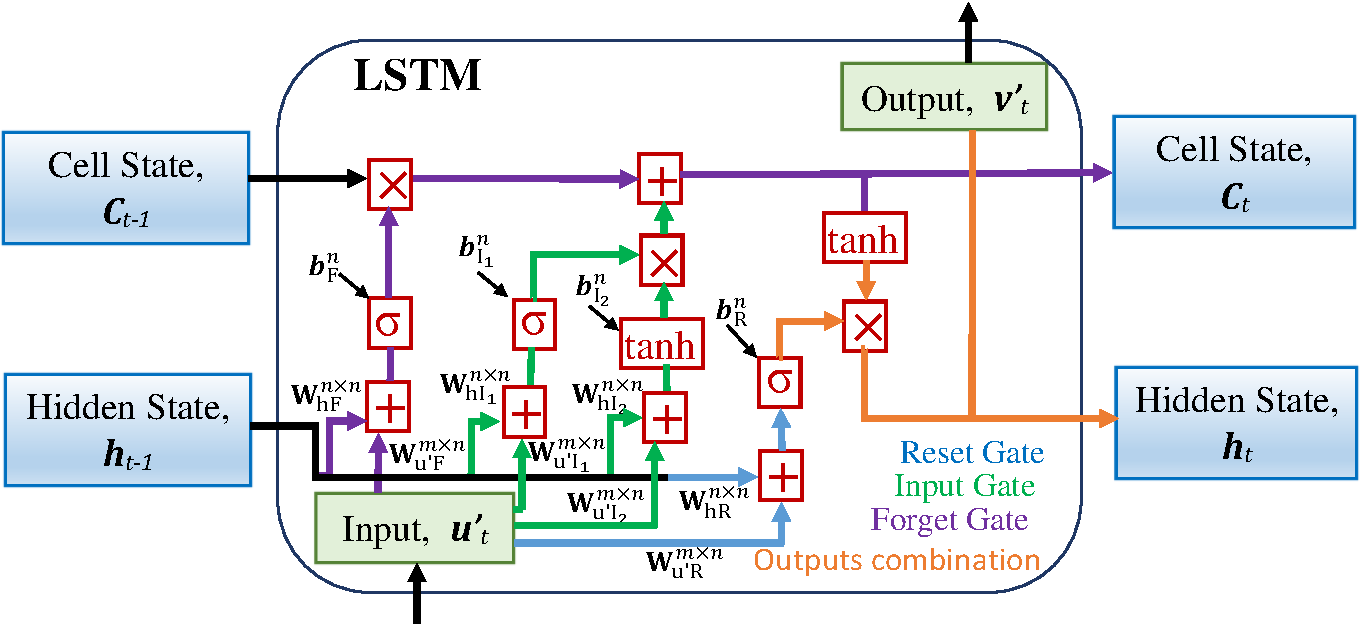
\includegraphics[width=\textwidth]{LSTM_detail}
	\end{subfigure}
	\caption{Detailed LSTM architecture outlining the path of information inside the module. The input vector $ \textit{\textbf{u}}' $ is of dimension $ m $, while the output vector $ \textit{\textbf{v}'} $, the hidden variable vector $ \textit{\textbf{h}} $ and the cell state vector $ \textit{\textbf{C}} $ are of dimension $ n $. The weight matrices $ \textbf{W}^{n\times n}_\text{h} $ and $ \textbf{W}^{m\times n}_\text{u'} $ act on the hidden state variable and input vector respectively with the subscripts F, I and R corresponding to the applied variables in the forget, input and the reset path respectively. Illustration inspired from \cite{UnderstandingLSTMNetworks}.}\label{app-lstm-detail}
\end{figure}

The operation symbols used in Figure \ref{app-lstm-detail} have the following implications:
\begin{itemize}
	\item $ \boxed{+} $: the element-wise summation operator of two vectors of same dimension, expressed as $ \textit{\textbf{r}}=\textit{\textbf{x}}+\textbf{\textit{y}} $;
	\item $ \boxed{\times} $: the element-wise product (Hadamard product) operator on two vectors of same dimension, expressed as $ r_i=x_iy_i $;
	\item $ \boxed{\sigma} $: the sigmoid activation functions;
	\item $ \boxed{\text{tanh}} $: the hyperbolic tangent activation function.
\end{itemize}

The detailed working of an LSTM cell as illustrated in Figure \ref{app-lstm-detail} can be summarized as follows:
\begin{itemize}
	\item The cell state $ \textbf{\textit{C}} $ runs like a conveyor belt along the cell with very minor interactions with the other paths. This lets information pass through with little modifications. By the controlling of specific gates, information can be added or removed from the cell state;
	\item The purple line comprises of the ``forget gate" where a sigmoid layer decides what information is to be thrown or ``forgotten" from the cell state by looking at the hidden variable coming from previous time step $ \textbf{\textit{h}}_{t-1} $ and the input vector $ \textit{\textbf{u}}_t $ before outputting a 0 or 1 in the forget vector $ \textbf{\textit{f}}_t $ for each number in cell state $ \textbf{\textit{C}}_{t-1} $. This operation can be written as 
	\begin{equation}\label{app-lstm-1}
	\textbf{\textit{f}}_t = \sigma(\textbf{W}^{n\times n}_{hF}\textbf{\textit{h}}_{t-1}+\textbf{W}^{n\times m}_{u'F}\textbf{\textit{u}}'_{t}+\textbf{\textit{b}}^n_F);
	\end{equation}	
	\item The green line decides what information will be stored in the cell state. This is comprised of two lines, a sigmoid ``input gate layer" that decides which values will be updated giving an input vector $ \textbf{\textit{i}}_t $ and a tanh layer that will create a list of new candidate values $ \tilde{\textbf{\textit{C}}}_t $. These operations can be written as
	\begin{equation}\label{app-lstm-2}
	\textbf{\textit{i}}_t = \sigma(\textbf{W}^{n\times n}_{hI_1}\textbf{\textit{h}}_{t-1}+\textbf{W}^{n\times m}_{u'I_1}\textbf{\textit{u}}'_{t}+\textbf{\textit{b}}^n_{I_1})
	\end{equation}
	and
	\begin{equation}\label{app-lstm-3}
	\tilde{\textbf{\textit{C}}}_t = \tanh(\textbf{W}^{n\times n}_{hI_2}\textbf{\textit{h}}_{t-1}+\textbf{W}^{n\times m}_{u'I_2}\textbf{\textit{u}}'_{t}+\textbf{\textit{b}}^n_{I_2});
	\end{equation}
	\item The purple line and the green line can be used to now update the old cell state $ \textbf{\textit{C}}_{t-1} $ into the new cell state $ \textbf{\textit{C}}_t $. The old state is multiplied by $ \textbf{\textit{f}}_t $ to ``forget" some values and then the element-wise product $ \textbf{\textit{i}}_t\odot\tilde{\textbf{\textit{C}}} $ is added to update the new candidate values by scaling them appropriately. This operation can be written as 
	\begin{equation}\label{app-lstm-4}
	\textbf{\textit{C}}_t = \textbf{\textit{f}}_t\odot\textbf{\textit{C}}_{t-1}+\textbf{\textit{i}}_t\odot\tilde{\textbf{\textit{C}}};
	\end{equation}
	\item The blue line denotes the reset gate layer that will decide what parts of cell state will be output in the output gate vector $ \textbf{\textit{o}}_t $. This layer has a sigmoid gate that can be written as
	\begin{equation}\label{app-lstm-5}
	\textbf{\textit{o}}_t=\sigma(\textbf{W}^{n\times n}_{hR}\textbf{\textit{h}}_{t-1}+\textbf{W}^{n\times m}_{u'R}\textbf{\textit{u}}'_{t}+\textbf{\textit{b}}^n_{R});
	\end{equation}
	\item The final operation to produce the output is denoted by the orange line where the cell state $ \textbf{\textit{C}}_t $ is put through a tanh layer and then multiplied by the output of the reset layer to give the final new hidden state $ \textbf{\textit{h}}_t $. This operation can be written as 
	\begin{equation}\label{app-lstm-6}
	\textbf{\textit{h}}_t=\textbf{\textit{o}}_t\odot\tanh(\textbf{\textit{C}}_t). 
	\end{equation}
	The new hidden variable $ \textbf{\textit{h}}_t $ is also the final output vector $ \textbf{\textit{v}}_t $.
\end{itemize}

Initially, at time $ t=0 $, both the cell state $ \textbf{\textit{C}}_0 $ and the hidden variable $ \textbf{\textit{h}}_0 $ are initialized to $ \bm0 $ value. However, a custom value can always be initialized to study the training behavior.

\paragraph*{Gated Recurrent Unit (GRU)} A simpler variant of an LSTM module is the GRU where the forget and the input gates have been merged to obtain a single ``update gate". The cell state and the hidden state are also merged\cite{choLearningPhraseRepresentations2014}(Figure \ref{app-lstm-gru}).

\begin{figure}
	\centering
	\begin{subfigure}{0.98\textwidth}
		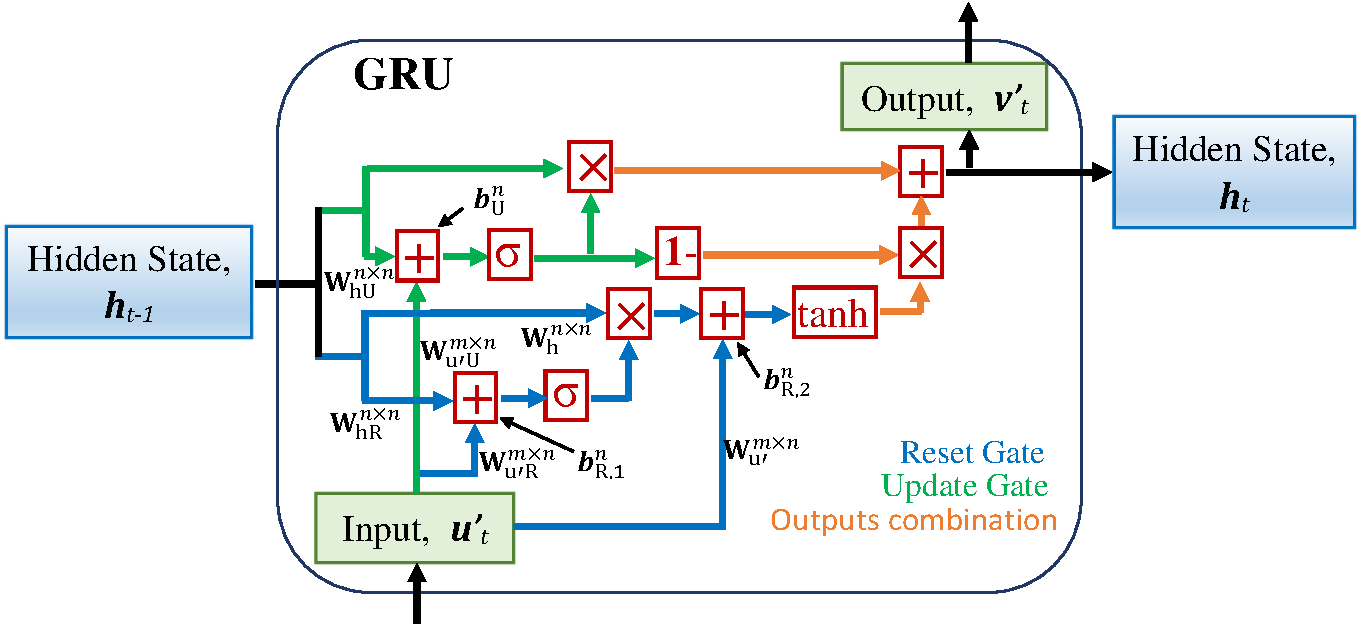
\includegraphics[width=\textwidth]{GRU_detail}
	\end{subfigure}
	\caption{Detailed GRU architecture outlining the path of information inside the module. The input vector $ \textit{\textbf{u}}' $ is of dimension $ m $, while the output vector $ \textit{\textbf{v}'} $ and the hidden variable vector $ \textit{\textbf{h}} $ are of dimension $ n $. The weight matrices $ \textbf{W}^{n\times n}_\text{h} $ and $ \textbf{W}^{m\times n}_\text{u'} $ act on the hidden state variable and input vector respectively with the subscripts U and R corresponding to the applied variables in the update and the reset path respectively. Image sourced from \cite{wuRecurrentNeuralNetworkaccelerated2020}.}\label{app-lstm-gru}
\end{figure}

In addition to the previously explained operative symbols, for the illustration in Figure \ref{app-lstm-gru}, the following one needs to be defined for GRU modules:
\begin{itemize}
	\item $ \boxed{\bm1-} $: element-wise operator on vector $ \textit{\textbf{x}} $ that performs the operation $ \textbf{\textit{r}}=\bm1-\textbf{\textit{x}} $.
\end{itemize}

The internal architecture of the GRU  Figure \ref{app-lstm-gru} can be summarized as follows:
\begin{itemize}
	\item The green line comprises the ``update gate", and this is analogous to the combination of the ``forget gate" and the ``input gate" in an LSTM module. A sigmoid layer looks at the hidden variable coming from the previous time step $ \textbf{\textit{h}}_{t-1} $ and the input vector $ \textbf{\textit{u}}_t $ to give the update vector $ \textbf{\textit{z}}_t $. This operation can be written as 
	\begin{equation}\label{app-lstm-gru-1}
	\textbf{\textit{z}}_t = \sigma(\textbf{W}^{n\times n}_{hU}\textbf{\textit{h}}_{t-1}+\textbf{W}^{n\times m}_{u'U}\textbf{\textit{u}}'_{t}+\textbf{\textit{b}}^n_{U});
	\end{equation}
	\item The blue line displays the reset gate that applies a sigmoid layer on the hidden variables from the previous time step $ \textbf{\textit{h}}_{t-1} $ and the input variable $ \textbf{\textit{u}}_t $ which will decide the values in the hidden variables from the previous time step that will be replaced with the vector of new values stored in the reset vector $ \textbf{\textit{r}}_t $. This operation can be written as 
	\begin{equation}\label{app-lstm-gru-2}
	\textbf{\textit{r}}_t = \sigma(\textbf{W}^{n\times n}_{hR}\textbf{\textit{h}}_{t-1}+\textbf{W}^{n\times m}_{u'R}\textbf{\textit{u}}'_{t}+\textbf{\textit{b}}^n_{R,1});
	\end{equation}
	\item The third layer is a tanh gate that creates a vector of candidate hidden values $ \tilde{\textbf{\textit{h}}}_t $ by looking at the input vector $ \textbf{\textit{u}}_t $ and the previous hidden state $ \textbf{\textit{h}}_{t-1} $ weighted by the output of the reset gate $ \textbf{\textit{r}}_t $. This operation can be written as
	\begin{equation}\label{app-lstm-gru-3}
	\tilde{\textbf{\textit{h}}}_t = \tanh(\textbf{W}^{n\times n}_{h}(\textbf{\textit{r}}_t\odot \textbf{\textit{h}}_{t-1})+\textbf{W}^{n\times m}_{u'}\textbf{\textit{u}}'_{t}+\textbf{\textit{b}}^n_{R,2});
	\end{equation}
	\item The orange line is the output combination line, and unlike an LSTM cell there is no gate working on this path. The candidate vector $ \tilde{\textbf{\textit{h}}}_t $ is weighted with the output of the ``update gate" treated with an element-wise $ \boxed{\bm1-} $ operation, $ \bm1-\textbf{\textit{z}}_t $ added to the hidden variable of the previous time step $ \textbf{\textit{h}}_{t-1} $ weighted by the output of the ``update gate" $ \textbf{\textit{z}}_t $ which result in the final hidden variable $ \textbf{\textit{h}}_t $. This operation can be written as
	\begin{equation}\label{app-lstm-gru-4}
	\textbf{\textit{h}}_t = \textbf{\textit{z}}_t\odot\textbf{\textit{h}}_{t-1}+(\bm1-\textbf{\textit{z}}_t)\odot\tilde{\textbf{\textit{h}}}_t.
	\end{equation}
	The new hidden variable $ \textbf{\textit{h}}_t $ is also the final output vector $ \textbf{\textit{v}}_t $.
	
\end{itemize}

